\usepackage{xcolor}
\usepackage{afterpage}
\usepackage{pifont,mdframed}
\usepackage[bottom]{footmisc}
\usepackage{minted}

\createsection{\Grader}{Grader di prova}
\newcommand{\inputfile}{\texttt{stdin}}
\newcommand{\outputfile}{\texttt{stdout}}
\makeatletter
\renewcommand{\this@inputfilename}{\texttt{stdin}}
\renewcommand{\this@outputfilename}{\texttt{stdout}}
\renewcommand{\this@syllabuslevel}{5}
\renewcommand{\this@custdifficulty}{3}
\makeatother
\setdifficulty{4}

% % % % % % % % % % % % % % % % % % % % % % % % % % % % % % % % % % % % % % % % % % %
% % % % % % % % % % % % % % % % % % % % % % % % % % % % % % % % % % % % % % % % % % %
L'allevatore Abbondanzio vuole costruire un recinto per le sue anatre, e perimetrarlo con delle corde.
Per fare ciò si è recato su Amazon e ha aquistato N corde diverse, dove la corda $i = 0 \dots N-1$ è lunga $V_i$ metri.
In particolare, il perimetro del recinto di Abbondanzio sarà lungo $K$ metri, perciò è necessaria una corda lunga $K$
oppure un suo multiplo, dato che una corda troppo lunga o troppo corta potrebbe rappresentare un pericolo per le sue anatre.

\begin{figure}[h]
    \centering
    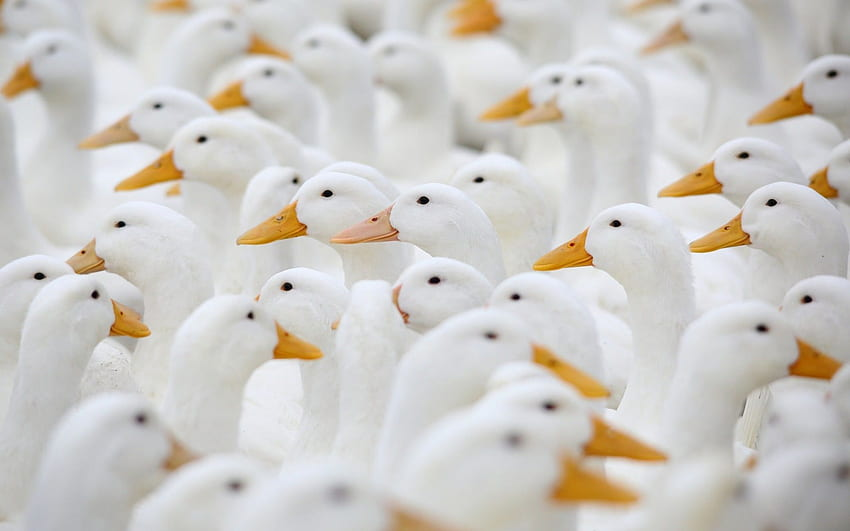
\includegraphics[width=0.5\textwidth]{duck.jpg}
    \caption{Anatre. Tante anatre.}
\end{figure}

Sfortunatamente le corde non sono tutte della lunghezza giusta, perciò vuole sceglierne $4$ e legarle insieme,
in modo che la lunghezza finale della corda sia $V_f = V_a + V_b + V_c + V_d$ metri.
Abbondanzio si è reso conto che ci sono molti modi per creare una corda adatta, e vuole sapere esattamente in quanti modi si può fare.

Più formalmente, dato un array $V$ di lunghezza $N$, trova in quanti modi puoi sceglere $4$ indici $a < b < c < d$ tali che
$V_a + V_b + V_c + V_d = K \cdot x$, dove $x$ è un intero maggiore di 0.


\Implementation

Dovrai sottoporre un unico file, con estensione \texttt{.cpp}.

\begin{warning}
    Tra gli allegati a questo task troverai un template \texttt{recinto.cpp} con un esempio di implementazione.
\end{warning}

Il file di input è composto da $2$ righe:
\begin{itemize}
    \item Riga 1: gli interi $N$ e $K$, separati da uno spazio.
    \item Riga 2: $N$ interi, ovvero le lunghezze delle corde separate da uno spazio.
\end{itemize}

Il file di output è composto da $1$ riga:
\begin{itemize}
    \item Riga 1: la risposta al problema.
\end{itemize}

% % % % % % % % % % % % % % % % % % % % % % % % % % % % % % % % % % % % % % % % % % %
% % % % % % % % % % % % % % % % % % % % % % % % % % % % % % % % % % % % % % % % % % %

\Constraints

\begin{itemize}[nolistsep, itemsep=2mm]
    \item $4 \le N \le 1\:000$.
    \item $2 \le K \le 1\:000\:000$.
    \item $1 \le V_i \le 1\:000\:000$, per ogni $i = 0 \dots N-1$.
\end{itemize}

% % % % % % % % % % % % % % % % % % % % % % % % % % % % % % % % % % % % % % % % % % %
% % % % % % % % % % % % % % % % % % % % % % % % % % % % % % % % % % % % % % % % % % %

\Scoring

Il tuo programma verrà testato su diversi test case raggruppati in subtask.
Per ottenere il punteggio relativo ad un subtask,
è necessario risolvere correttamente tutti i test che lo compongono.

\IIOTsubtask{0}{1}{Casi d'esempio.}

\IIOTsubtask{10}{1}{$N \le 30$ e $K \le 30$.}

\IIOTsubtask{15}{1}{$N \le 30$.}

\IIOTsubtask{20}{3}{$K \le 30$.}

\IIOTsubtask{55}{3}{Nessuna limitazione aggiuntiva.}


% % % % % % % % % % % % % % % % % % % % % % % % % % % % % % % % % % % % % % % % % % %
% % % % % % % % % % % % % % % % % % % % % % % % % % % % % % % % % % % % % % % % % % %

\Examples

\begin{example}
    \exmpfile{recinto.input0.txt}{recinto.output0.txt}%
\end{example}

% % % % % % % % % % % % % % % % % % % % % % % % % % % % % % % % % % % % % % % % % % %
% % % % % % % % % % % % % % % % % % % % % % % % % % % % % % % % % % % % % % % % % % %

\Explanation

Nel caso d'esempio, ci sono $4$ combinazioni valide: $(3, 10, 4, 3), (3, 10, 1, 2), (3, 4, 3, 2), (10, 3, 1, 2)$.

Nota che due corde della stessa lunghezza possono essere legate tra di loro. Possono anche formare combinazioni diverse,
come ad esempio $(3, 10, 1, 2)$ che compare due volte perché ci sono due corde diverse di lunghezza 3.